\chapter{Kiến trúc hệ thống đề xuất}

\section{Tổng quan kiến trúc hệ thống}

Hệ thống Edge-AI được thiết kế dựa trên kiến trúc không đồng nhất 
(Heterogeneous Architecture) của nền tảng Zynq UltraScale+ MPSoC trên bo mạch Kria KV260. 
Thiết kế tận dụng mô hình đồng thiết kế phần cứng/phần mềm (Hardware/Software Co-design)
 để tối ưu hóa hiệu năng xử lý.

\begin{figure}[!h]
\centering
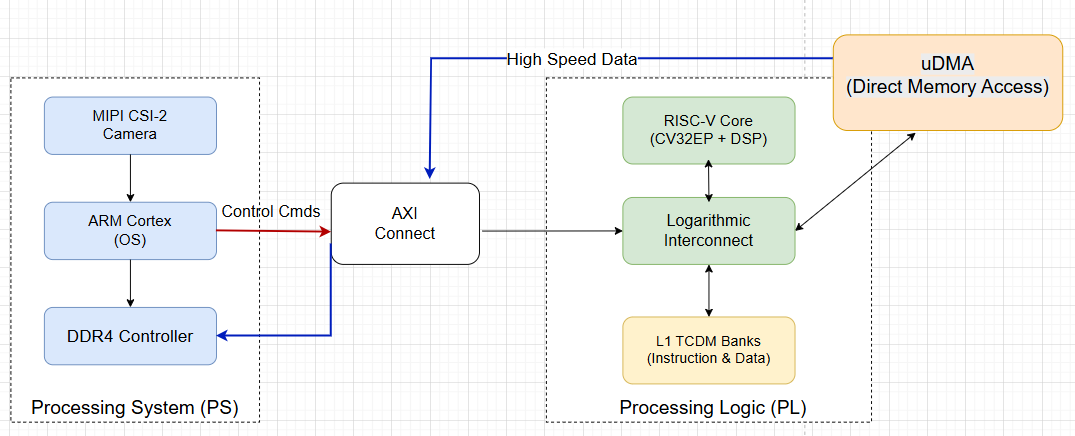
\includegraphics[width=1\textwidth]{images/design/arch.png}
\caption{Kiến trúc hệ thống tổng quan}
\label{fig:proposed_architecture}
\end{figure}

Mô hình tổng thể được chia thành hai miền xử lý chính:
\begin{itemize}
    \item Processing System
    \item Khối Cầu nối
    \item Programmable Logic
\end{itemize}

Như thể hiện tại Hình \ref{fig:proposed_architecture}, hệ thống được phân chia thành ba miền xử lý chính với các vai trò chuyên biệt:

\begin{itemize}
    \item \textbf{Phân hệ Xử lý (Processing System - PS):} 
    Đóng vai trò là khối điều khiển trung tâm (Host), hoạt động trên nền tảng vi xử lý ARM Cortex-A53 lõi tứ. PS chịu trách nhiệm:
    \begin{itemize}
        \item Quản lý tài nguyên hệ thống và khởi chạy quy trình boot.
        \item Giao tiếp với các ngoại vi tiêu chuẩn như Camera (qua giao diện MIPI CSI-2) và Màn hình.
        \item Thực hiện các bước tiền xử lý hình ảnh (Preprocessing) và quản lý bộ nhớ đệm dữ liệu (Data Buffering) trên DDR4.
    \end{itemize}

    \item \textbf{Khối Giao tiếp Liên kết (Interconnect Fabric):} 
    Đóng vai trò là cầu nối dữ liệu tốc độ cao, sử dụng giao thức chuẩn công nghiệp AMBA AXI4. Khối này bao gồm các bộ chuyển mạch thông minh (AXI SmartConnect) để:
    \begin{itemize}
        \item Phân tách luồng điều khiển (Control Plane) băng thông thấp và luồng dữ liệu (Data Plane) băng thông cao.
        \item Đảm bảo đồng bộ hóa giữa hai miền xung nhịp khác nhau của PS và PL.
        \item Cho phép truy cập bộ nhớ chia sẻ (Shared Memory) một cách trong suốt giữa các vi xử lý.
    \end{itemize}

    \item \textbf{Phân hệ Logic Khả trình (Programmable Logic - PL):} 
    Đóng vai trò là bộ tăng tốc tính toán (Accelerator). Tại đây, tài nguyên FPGA được cấu hình để triển khai một Hệ thống trên Chip (SoC) con, bao gồm:
    \begin{itemize}
        \item \textbf{Lõi vi xử lý mềm RISC-V (PULP Subsystem):} Điều phối luồng thực thi thuật toán AI.
        \item \textbf{Bộ tăng tốc phần cứng (CNN Accelerator):} Thực hiện các phép toán tích chập chuyên sâu.
        \item \textbf{Cơ chế truy cập bộ nhớ trực tiếp (uDMA):} Tối ưu hóa việc di chuyển dữ liệu ảnh mà không làm gián đoạn CPU.
    \end{itemize}
\end{itemize}

Sự kết hợp chặt chẽ giữa ba thành phần này cho phép hệ thống hoạt động theo cơ chế đường ống (Pipelining), đảm bảo khả năng xử lý hình ảnh thời gian thực với độ trễ thấp nhất.

%=======================================================================
\newpage
\section{Thiết kế Processing System}

Đây là phần cứng có sẵn (Hard-core) trên chip Zynq UltraScale+ của board Kria KV260.
\begin{itemize}
    \item ARM Cortex-A53: Đóng vai trò là CPU chủ (Host). Nó có thểchạy hệ điều hành (Linux hoặc Bare-metal) 
để quản lý toàn bộ hệ thống. Nhiệm vụ của nó là giao tiếp với Camera (qua cổng MIPI), 
nhận ảnh, tiền xử lý (resize, crop) và lưu trữ ảnh vào bộ nhớ lớn.
    \item DDR4 Controller (Shared Memory): Đây là kho chứa dữ liệu chung. Vì bộ nhớ trong của RISC-V 
rất nhỏ (chỉ vài chục KB), toàn bộ dữ liệu ảnh đầu vào (Image Buffer) phải được lưu ở đây 
(4GB RAM của Kria).
\end{itemize}

PS đóng vai trò "Master" điều phối, gửi lệnh "Bắt đầu" (Start) cho khối PL 
khi đã có dữ liệu ảnh sẵn sàng.

\subsection{Sơ đồ cấu hình khối Zynq UltraScale+ (PS Block Design)}

\begin{figure}[!h]
    \centering
    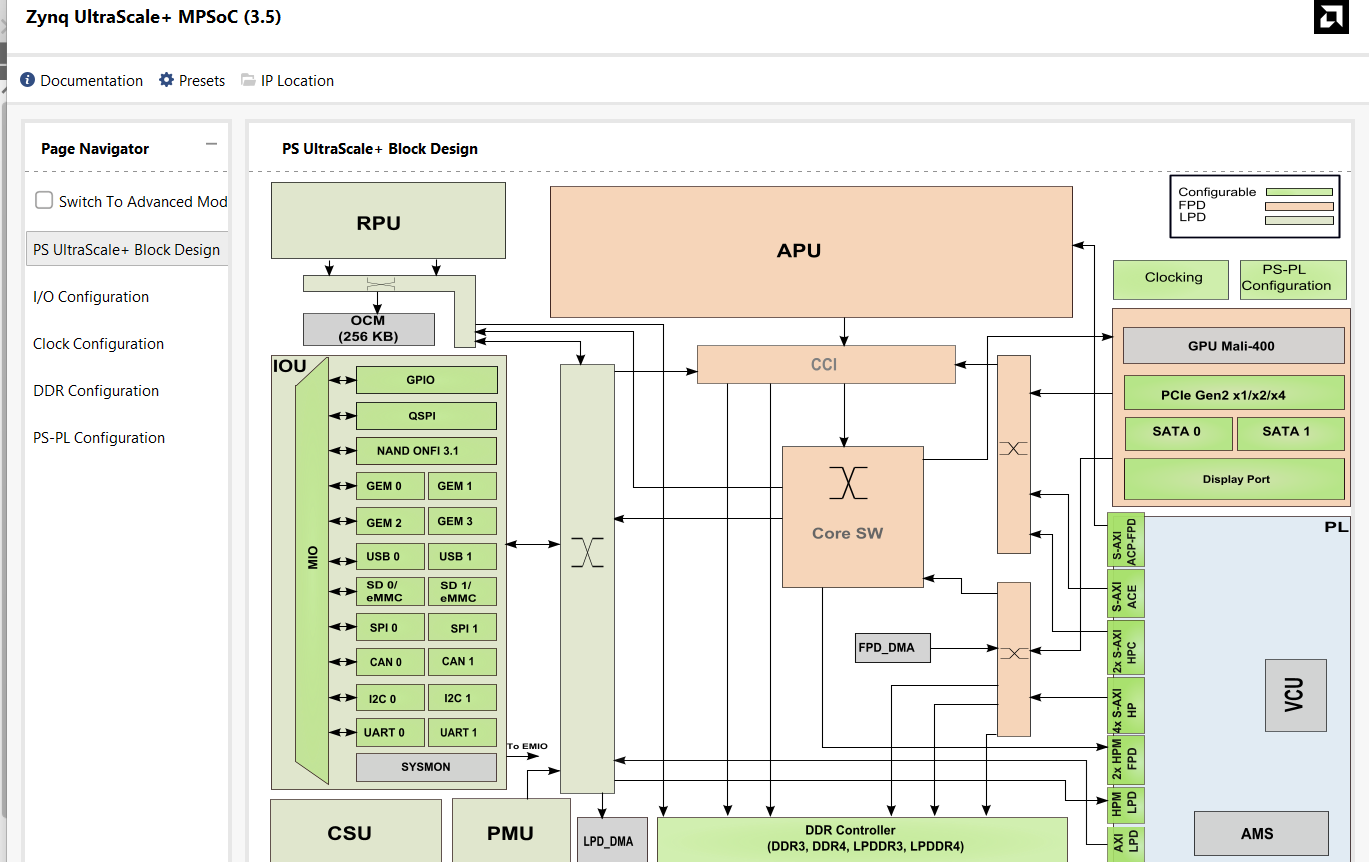
\includegraphics[width=1\textwidth]{images/design/zynq.png}  
    \caption{Sơ đồ cấu hình khối Zynq UltraScale+ MPSoC trên Vivado.}
    \label{fig:ps_block_design}
\end{figure}

\subsection{Cấu hình chi tiết các phân hệ}

\subsubsection{Khối xử lý ứng dụng (APU Configuration)}
Trung tâm của PS là cụm vi xử lý Quad-core ARM Cortex-A53 hoạt động ở tần số 1.2 GHz. Trong thiết kế này, APU được cấu hình để:
\begin{itemize}
    \item \textbf{Chế độ hoạt động:} Chạy hệ điều hành PetaLinux (dựa trên Yocto Project) để tận dụng các driver có sẵn cho Camera MIPI và ngăn xếp mạng (Network Stack).
    \item \textbf{Quản lý Boot:} Sử dụng giao diện SD Card (SD1) kết nối với các chân MIO để nạp bitstream cho FPGA và khởi động hệ thống.
\end{itemize}

\subsubsection{Cấu hình Giao diện Bộ nhớ (DDR Configuration)}
Bộ điều khiển DDR4 (DDRC) được kích hoạt để quản lý 4GB RAM tích hợp trên Kria SOM. Cấu hình này rất quan trọng vì nó đóng vai trò là "Shared Memory" cho cả hệ thống:
\begin{itemize}
    \item \textbf{Data Width:} 64-bit (hỗ trợ băng thông cao).
    \item \textbf{AXI Port QoS:} Cổng S\_AXI\_HP0 được ưu tiên mức Quality of Service (QoS) cao để đảm bảo uDMA không bị nghẽn khi ghi dữ liệu ảnh, tránh hiện tượng rớt khung hình (frame drop).
\end{itemize}

\subsubsection{Cấu hình Giao diện PS-PL (Interface Configuration)}
Để kết nối với miền Logic khả trình (nơi chứa RISC-V và Accelerator), hai cổng giao tiếp AXI quan trọng được kích hoạt:

\begin{enumerate}
    \item \textbf{M\_AXI\_HPM0\_FPD (Master):}
    \begin{itemize}
        \item \textit{Chức năng:} Cổng Master hiệu năng cao miền công suất thấp (Full Power Domain).
        \item \textit{Nhiệm vụ:} Dùng để CPU ARM gửi tín hiệu điều khiển, cấu hình thanh ghi và nạp firmware vào bộ nhớ lệnh của RISC-V.
        \item \textit{Độ rộng:} 32-bit (phù hợp với bus AXI-Lite).
    \end{itemize}
    
    \item \textbf{S\_AXI\_HP0\_FPD (Slave):}
    \begin{itemize}
        \item \textit{Chức năng:} Cổng Slave hiệu năng cao (High Performance).
        \item \textit{Nhiệm vụ:} Cho phép các Master bên phía FPGA (cụ thể là uDMA) truy cập trực tiếp vào RAM DDR4.
        \item \textit{Độ rộng:} 128-bit (để tối đa hóa tốc độ truyền tải ảnh).
    \end{itemize}
\end{enumerate}

\subsubsection{Cấu hình Xung nhịp (Clock Configuration)}
Khối PS cung cấp nguồn xung nhịp tham chiếu cho toàn bộ logic bên phía PL 
thông qua chân \texttt{pl\_clk0}. Tần số được thiết lập là \textbf{100 MHz}, 
đảm bảo sự cân bằng giữa tốc độ xử lý của nhân RISC-V và mức tiêu thụ năng lượng.

%=========================================================
\newpage
\section{Thiết kế Hệ thống Giao tiếp và Bộ nhớ (Interconnect \& Memory Hierarchy)}
\label{sec:interconnect_design}

Trong kiến trúc SoC dị thể, hiệu năng của hệ thống không chỉ phụ thuộc vào tốc độ xử lý của từng nhân (Core) mà còn phụ thuộc vào băng thông và độ trễ của hệ thống kết nối. Mục này trình bày thiết kế chi tiết mạng lưới giao tiếp giữa PS và PL, cùng với quy hoạch không gian bộ nhớ chung.

\begin{figure}[h]
    \centering
    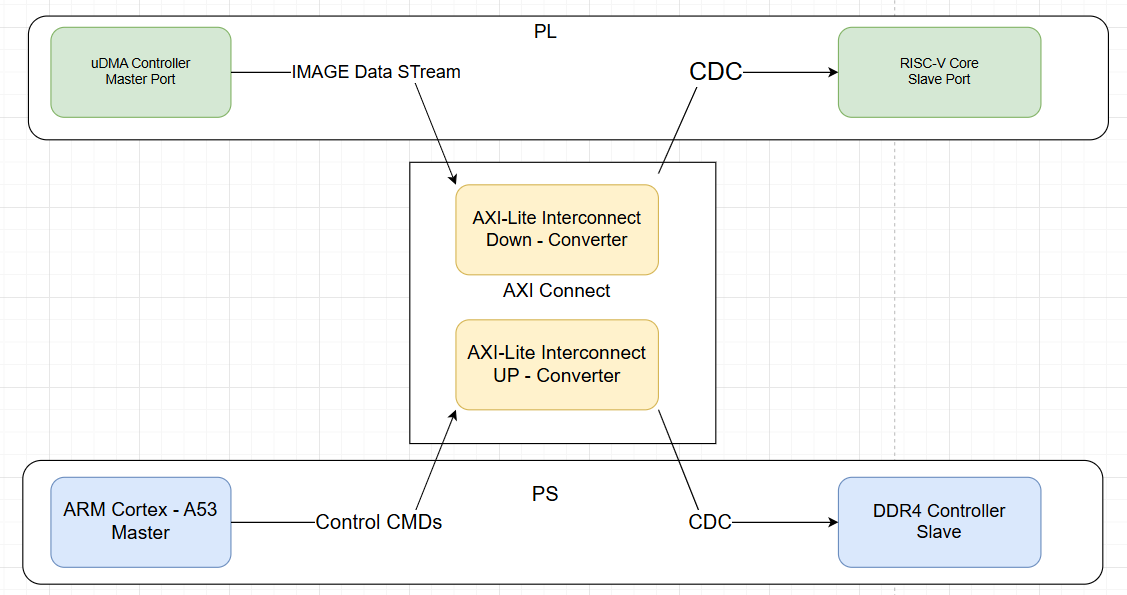
\includegraphics[width=1\textwidth]{images/design/axi_arch.png}  
    \caption{Sơ đồ khối hệ thống giao tiếp AXI giữa PS và PL.}
    \label{fig:axi_interconnect}
\end{figure}


\subsection{Cơ chế AXI SmartConnect (PS-PL Bridge)}
Để kết nối miền xử lý ứng dụng (PS) hoạt động ở tần số cao và miền logic khả trình (PL) hoạt động ở tần số thấp, hệ thống sử dụng khối IP **AXI SmartConnect**. Đây không chỉ là dây dẫn đơn thuần mà là một ma trận chuyển mạch thông minh (Switch Fabric) đảm nhiệm ba chức năng:
\begin{itemize}
    \item \textbf{Clock Domain Crossing (CDC):} Đồng bộ hóa tín hiệu giữa miền xung nhịp PS (1.2 GHz) và miền PL (100 MHz) bằng các bộ đệm FIFO bất đồng bộ, đảm bảo không xảy ra lỗi Metastability.
    \item \textbf{Width Conversion:} Chuyển đổi độ rộng dữ liệu tự động giữa bus hệ thống 128-bit (phía DDR) và bus ngoại vi 32-bit (phía RISC-V).
    \item \textbf{Arbitration:} Phân giải tranh chấp khi nhiều Master cùng truy cập bộ nhớ.
\end{itemize}

Hệ thống được thiết kế với hai kênh giao tiếp vật lý tách biệt:

\subsubsection{Kênh Điều khiển (Control Path - AXI4-Lite)}
Đây là tuyến giao tiếp từ \textbf{Master (ARM Cortex-A53)} đến \textbf{Slave (PULP Subsystem)}.
\begin{itemize}
    \item \textbf{Giao thức:} AXI4-Lite 32-bit. Đây là phiên bản rút gọn của AXI4, không hỗ trợ truyền tải dạng Burst.
    \item \textbf{Mục đích:} Tối ưu hóa cho các giao dịch đơn lẻ, độ trễ thấp.
    \item \textbf{Chức năng:} Dùng để CPU ARM thực hiện các tác vụ quản trị như:
    \begin{itemize}
        \item Cấu hình thanh ghi điều khiển của bộ tăng tốc CNN (Trọng số, Bias, Kích thước ảnh).
        \item Gửi tín hiệu kích hoạt (Trigger) quá trình suy luận.
        \item Reset mềm (Soft-reset) khối PL trong trường hợp treo hệ thống.
    \end{itemize}
\end{itemize}

\subsubsection{Kênh Dữ liệu (Data Path - AXI4-Full)}
Đây là tuyến giao tiếp từ \textbf{Master (uDMA Controller)} đến \textbf{Slave (DDR4 Controller)}.
\begin{itemize}
    \item \textbf{Giao thức:} AXI4-Full 128-bit.
    \item \textbf{Mục đích:} Tối ưu hóa băng thông (Throughput).
    \item \textbf{Chức năng:} Hỗ trợ cơ chế \textit{Burst Transaction}, cho phép uDMA đọc/ghi liên tiếp tới 256 gói dữ liệu chỉ với một địa chỉ bắt đầu. Điều này cực kỳ quan trọng để đảm bảo cung cấp đủ dữ liệu pixel cho mạng MobileNet hoạt động thời gian thực (Real-time).
\end{itemize}

\subsection{Quy hoạch không gian bộ nhớ (System Memory Map)}
Do RISC-V Soft-core sử dụng kiến trúc bộ nhớ phẳng (Flat Memory Model) 32-bit, việc phân chia địa chỉ phải được thiết kế cẩn trọng để map chính xác với địa chỉ vật lý của hệ thống Zynq.

Bảng \ref{tab:memory_map} mô tả bản đồ bộ nhớ từ góc nhìn của vi xử lý RISC-V:

\begin{table}[h]
\centering
\caption{Bản đồ bộ nhớ hệ thống (System Memory Map)}
\label{tab:memory_map}
\begin{tabular}{|l|l|l|p{5cm}|}
\hline
\textbf{Vùng nhớ} & \textbf{Địa chỉ (Base)} & \textbf{Kích thước} & \textbf{Chức năng chi tiết} \\ \hline
\texttt{INSTR\_RAM} & \texttt{0x0000\_0000} & 64 KB & Bộ nhớ chứa Firmware. Khi Reset, RISC-V sẽ trỏ PC (Program Counter) vào đây. \\ \hline
\texttt{DATA\_RAM} & \texttt{0x0010\_0000} & 64 KB & Vùng nhớ TCDM cục bộ, chứa Stack, Heap và biến cục bộ. Truy cập trong 1 chu kỳ. \\ \hline
\texttt{PERIPHERAL} & \texttt{0x1A10\_0000} & 4 KB & Vùng thanh ghi ngoại vi (MMIO) để điều khiển Timer, Event Unit và uDMA. \\ \hline
\textbf{\texttt{SHARED\_DDR}} & \textbf{\texttt{0x4000\_0000}} & \textbf{16 MB} & \textbf{Bộ nhớ chia sẻ (Shared Memory).} Được ánh xạ trực tiếp từ DDR4 của Zynq. Chứa Frame Buffer ảnh đầu vào và Output Tensor. \\ \hline
\texttt{MAILBOX} & \texttt{0xA000\_0000} & 4 KB & \textbf{Giao tiếp liên nhân (IPC).} Chứa các cờ hiệu (Semaphores) để đồng bộ trạng thái giữa ARM và RISC-V. \\ \hline
\end{tabular}
\end{table}

\subsubsection{Cơ chế Đồng bộ hóa (Mailbox Mechanism)}
Để tránh xung đột khi hai vi xử lý cùng truy cập vùng \texttt{SHARED\_DDR}, cơ chế Mailbox hoạt động như sau:
\begin{enumerate}
    \item \textbf{ARM:} Sau khi ghi ảnh vào DDR, ARM ghi giá trị \texttt{0x1} vào thanh ghi Mailbox để báo hiệu "Data Ready".
    \item \textbf{RISC-V:} Liên tục kiểm tra (Polling) hoặc nhận ngắt từ Mailbox. Khi thấy \texttt{0x1}, nó bắt đầu xử lý và ghi đè giá trị \texttt{0x2} ("Processing").
    \item \textbf{RISC-V:} Khi xử lý xong, ghi giá trị \texttt{0x3} ("Done").
    \item \textbf{ARM:} Đọc thấy \texttt{0x3}, lấy kết quả và reset Mailbox về \texttt{0x0}.
\end{enumerate}


%=============================================
%
%=============================================
\newpage
\section{Thiết kế Programmable Logic}
\label{sec:pl_design}

Logic Khả trình (PL) được thiết kế như một Hệ thống trên Chip (SoC) thu nhỏ hoạt động độc lập, dựa trên kiến trúc mở PULPissimo. Mục tiêu của phân hệ này là tạo ra một môi trường tính toán hiệu năng cao, độ trễ thấp để thực thi các tác vụ điều khiển và tăng tốc AI, giảm tải cho vi xử lý chính ARM.

\subsection{Kiến trúc tổng thể Phân hệ PULP (PULP Subsystem)}
Hình \ref{fig:pulp_arch} trình bày sơ đồ kiến trúc chi tiết của khối PL. Thiết kế bao gồm ba thành phần cốt lõi: Lõi xử lý RISC-V, Hệ thống bộ nhớ TCDM phân tán, và Bộ điều khiển uDMA, được kết nối với nhau thông qua một mạng lưới giao tiếp băng thông rộng (Logarithmic Interconnect).

\begin{figure}[h]
    \centering
    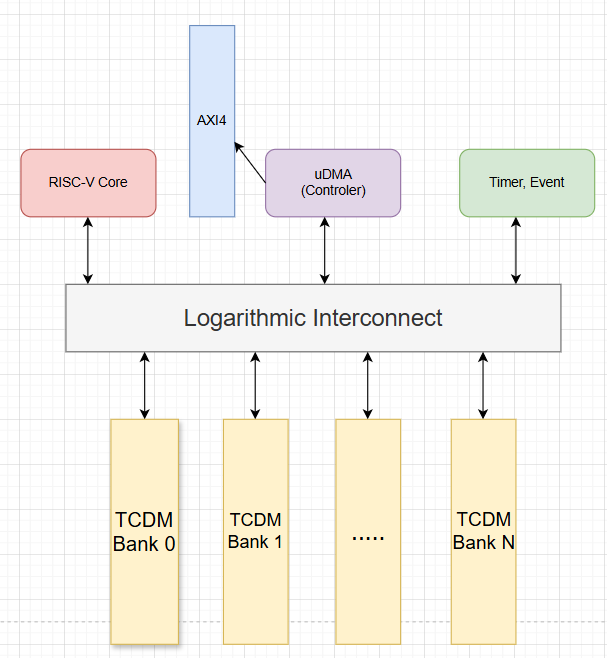
\includegraphics[width=0.8\textwidth]{images/design/pulp_arch.png}  
    \caption{Sơ đồ kiến trúc nội bộ của Phân hệ PULP trên FPGA.}
    \label{fig:pulp_arch}
\end{figure}

\subsection{Cấu hình Nhân Vi xử lý (RISC-V Core Configuration)}
Trung tâm điều khiển của PL là lõi IP RISC-V (dựa trên nhân CV32E40P). Lõi này được tham số hóa trước khi tổng hợp (Synthesis) để đạt sự cân bằng tối ưu giữa tài nguyên FPGA (LUTs) và hiệu năng tính toán:

\begin{table}[h]
\centering
\caption{Thông số cấu hình RISC-V Soft-core}
\label{tab:riscv_config}
\begin{tabular}{|l|l|p{6cm}|}
\hline
\textbf{Tham số} & \textbf{Giá trị} & \textbf{Ý nghĩa thiết kế} \\ \hline
Architecture & RV32IMCXpulp & Hỗ trợ tập lệnh nhân (M), nén (C) và mở rộng DSP/SIMD (Xpulp) cho AI. \\ \hline
Pipeline Stages & 4 & Đủ sâu để đạt tần số 100MHz, đủ ngắn để giảm độ trễ rẽ nhánh. \\ \hline
FPU & Disabled & Không sử dụng bộ xử lý dấu phẩy động để tiết kiệm diện tích (MobileNet đã được lượng tử hóa sang INT8). \\ \hline
Instruction Cache & 4 KB & Kiểu Direct Mapped, giúp CPU nạp lệnh nhanh mà không cần truy cập RAM ngoài liên tục. \\ \hline
Boot Address & \texttt{0x1A00\_0000} & Vị trí vector ngắt khởi động, trỏ tới vùng nhớ ROM khởi tạo. \\ \hline
\end{tabular}
\end{table}

\subsection{Hệ thống Bộ nhớ TCDM và Interconnect}
Điểm yếu chí tử của các hệ thống đa vi xử lý là hiện tượng tranh chấp bộ nhớ (Memory Contention). Thiết kế này giải quyết triệt để vấn đề trên bằng kiến trúc TCDM (Tightly Coupled Data Memory).

\subsubsection{Tổ chức Bộ nhớ Đan xen (Interleaved Memory Banking)}
Thay vì sử dụng một khối Block RAM khổng lồ đơn nhất (64KB), bộ nhớ TCDM được chia nhỏ thành \textbf{16 ngân hàng (Banks)}, mỗi ngân hàng có dung lượng 4KB.
\begin{itemize}
    \item \textbf{Nguyên lý:} Các địa chỉ liên tiếp nhau ($Addr, Addr+4, Addr+8...$) được lưu trữ lần lượt trên các Bank khác nhau ($Bank_0, Bank_1, Bank_2...$).
    \item \textbf{Lợi ích:} Cho phép truy cập song song. Ví dụ: RISC-V Core có thể đọc dữ liệu tại địa chỉ $A$ (nằm ở Bank 0) cùng lúc uDMA ghi dữ liệu vào địa chỉ $B$ (nằm ở Bank 1) mà không hề xảy ra xung đột.
\end{itemize}

\subsubsection{Logarithmic Interconnect}
Kết nối giữa các Master (Core, uDMA) và các Slave (Memory Banks) không phải là một Bus tuyến tính mà là một \textbf{Ma trận chuyển mạch (Switch Matrix)}.
\begin{itemize}
    \item Mạng lưới này có độ trễ cực thấp (chỉ 1 chu kỳ xung nhịp).
    \item Đảm bảo băng thông cực đại: Tổng băng thông nội bộ có thể đạt tới $N \times 32$-bit/cycle (với N là số lượng Bank).
\end{itemize}

\subsection{Cơ chế Truy cập Bộ nhớ Trực tiếp (uDMA)}
Để giải phóng CPU khỏi tác vụ sao chép dữ liệu nhàm chán, một bộ điều khiển uDMA (Micro-DMA) chuyên dụng được tích hợp:
\begin{itemize}
    \item \textbf{Chức năng:} uDMA đóng vai trò cầu nối giữa các ngoại vi tốc độ cao (như AXI4 port nối tới DDR4, SPI, Camera) và bộ nhớ TCDM.
    \item \textbf{Double Buffering:} uDMA hỗ trợ cấu hình hai vùng đệm (Buffer A và Buffer B). Khi đang xử lý dữ liệu ở Buffer A, uDMA sẽ tự động tải dữ liệu mới vào Buffer B trong nền (Background).
    \item \textbf{Kết nối với Accelerator:} uDMA cung cấp một luồng dữ liệu liên tục (Stream) cho khối tăng tốc CNN thông qua giao diện AXI-Stream, đảm bảo bộ tăng tốc luôn có dữ liệu để tính toán (tránh hiện tượng Starvation).
\end{itemize}

%=============================================================
\newpage
\section{Thiết kế Khối Tăng tốc phần cứng (CNN Accelerator)}
Nằm trong PL, khối tăng tốc CNN được thiết kế để thực hiện các phép toán tích chập
một cách song song và hiệu quả. Thiết kế này bao gồm các thành phần chính \cite{fpga2}
\label{sec:cnn_accelerator}

Đây là thành phần cốt lõi quyết định hiệu năng của toàn bộ hệ thống Edge-AI. 
Để đáp ứng yêu cầu tính toán thời gian thực của mạng MobileNetV1, nhóm thực hiện thiết kế một bộ tăng tốc phần cứng chuyên dụng (Domain-Specific Architecture - DSA) được tích hợp trong miền Logic khả trình (PL).
Khối tăng tốc này được thiết kế để giảm tải (offload) các phép toán tích 
chập nặng nề nhất khỏi vi xử lý RISC-V, hoạt động theo cơ chế dòng dữ liệu 
(Dataflow) để tối đa hóa thông lượng.

\subsection{Kiến trúc tổng quát khối Accelerator}
Sơ đồ khối chức năng của bộ tăng tốc được mô tả trong Hình \ref{fig:accel_arch}. Khối này giao tiếp với hệ thống thông qua hai giao diện chính:

\begin{figure}[h]
\centering
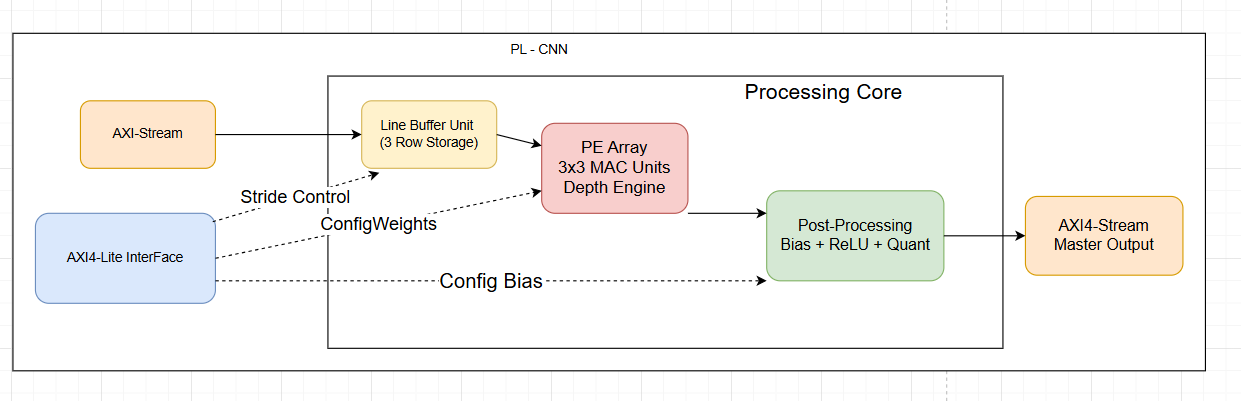
\includegraphics[width=1\textwidth]{images/design/cnn_acce.png}
\caption{Sơ đồ khối chức năng chi tiết của bộ tăng tốc CNN (Accelerator Core Architecture).}
\label{fig:accel_arch}
\end{figure}

\begin{itemize}
    \item \textbf{AXI4-Stream Slave:} Nhận dòng pixel ảnh đầu vào từ uDMA hoặc trực tiếp từ bộ nhớ đệm.
    \item \textbf{AXI4-Stream Master:} Đẩy dòng kết quả (Feature Maps) sau khi tính toán trở lại bộ nhớ.
\end{itemize}

\subsection{Các thành phần chức năng chi tiết}

\subsubsection{Bộ đệm dòng (Line Buffer Unit)}
Do đặc thù của phép tích chập $3 \times 3$ trong MobileNet, tại một thời điểm cần truy cập đồng thời các điểm ảnh thuộc 3 hàng liên tiếp. 
\begin{itemize}
    \item \textbf{Vấn đề:} Nếu đọc từ RAM từng pixel cho mỗi lần trượt cửa sổ, băng thông bộ nhớ sẽ bị quá tải.
    \item \textbf{Giải pháp:} Thiết kế sử dụng cơ chế \textit{Line Buffer} (Bộ đệm dòng) dựa trên BRAM nội bộ. Khi một pixel mới đi vào, nó đẩy các pixel cũ lên các hàng trên (Shift Register). Điều này cho phép tái sử dụng dữ liệu cục bộ, giảm nhu cầu truy cập RAM xuống 3 lần.
\end{itemize}

\subsubsection{Mảng tính toán (Processing Element Array - PE)}
Đây là trung tâm tính toán của Accelerator, được tối ưu cho phép \textbf{Tích chập tách biệt chiều sâu (Depthwise Convolution)}:
\begin{itemize}
    \item Cấu trúc bao gồm 9 bộ nhân (Multipliers) hoạt động song song, tương ứng với Kernel $3 \times 3$.
    \item Các phép toán được thực hiện trên định dạng số nguyên 8-bit (\texttt{int8}) để tiết kiệm tài nguyên DSP Slice trên FPGA.
    \item Kết quả của 9 phép nhân được cộng dồn (Accumulate) để tạo ra một điểm ảnh đầu ra trong mỗi chu kỳ xung nhịp (Single-cycle throughput).
\end{itemize}

\subsubsection{Khối xử lý phi tuyến và Lượng tử hóa (Post-Processing Unit)}
Sau khi tính tổng chập, dữ liệu cần đi qua các bước hậu xử lý trước khi xuất ra ngoài:
\begin{enumerate}
    \item \textbf{Bias Addition:} Cộng giá trị Bias (được nạp trước vào thanh ghi cấu hình).
    \item \textbf{ReLU Activation:} Áp dụng hàm kích hoạt $f(x) = max(0, x)$. Trên phần cứng, đây đơn giản là bộ so sánh với 0 (Multiplexer).
    \item \textbf{Re-Quantization:} Kết quả cộng dồn có thể lên tới 32-bit. Khối này thực hiện nhân với tỷ lệ (Scale factor) và dịch bit (Bit shift) để đưa dữ liệu trở về dạng 8-bit, sẵn sàng cho lớp mạng tiếp theo.
\end{enumerate}

\subsection{Tối ưu hóa cho MobileNetV1}
Thiết kế này giải quyết hai nút thắt chính của MobileNet trên phần cứng:
\begin{itemize}
    \item \textbf{Hỗ trợ Stride = 2:} Accelerator có logic điều khiển để tự động bỏ qua các pixel khi thực hiện giảm kích thước ảnh (Downsampling), giúp giảm 75\% khối lượng tính toán ở các lớp đầu của mạng.
    \item \textbf{Pipelining:} Toàn bộ quá trình từ nạp dữ liệu $\rightarrow$ Line Buffer $\rightarrow$ PE $\rightarrow$ ReLU $\rightarrow$ Xuất dữ liệu được thiết kế theo dạng đường ống (Pipeline). Khi ống đầy, hệ thống đạt hiệu suất 1 kết quả/1 chu kỳ xung nhịp.
\end{itemize}

%=============================================================
%
%=============================================================
\newpage
\section{Thuật toán AI và Thiết kế Phần mềm}
\label{sec:ai_algorithm}

Hệ thống được thiết kế để triển khai mạng nơ-ron tích chập \textbf{MobileNetV1}, 
một kiến trúc được tối ưu hóa cho các thiết bị di động với đặc trưng là sử dụng các 
lớp tích chập tách biệt theo chiều sâu (Depthwise Separable Convolution).

\subsection{Đặc tả Kiến trúc Mô hình}

\begin{figure}[!h]
\centering
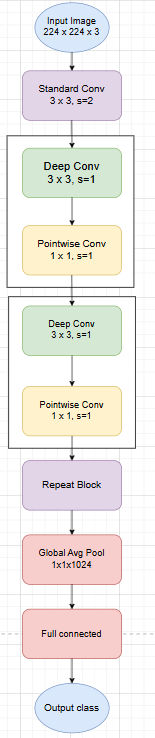
\includegraphics[width=0.2\textwidth]{images/design/conv.png}
\caption{Sơ đồ khối tích chập}
\label{fig:mobilenetv1_arch}
\end{figure}

\newpage

Mô hình được cấu hình với các siêu tham số (Hyperparameters) đầu vào như sau:
\begin{itemize}
    \item \textbf{Kích thước đầu vào (Input Shape):} $224 \times 224 \times 3$ (RGB Image).
    \item \textbf{Độ sâu màu (Bit-depth):} 8-bit Integer (sau khi lượng tử hóa).
    \item \textbf{Tổng số tham số (Parameters):} Xấp xỉ 4.2 triệu tham số.
    \item \textbf{Số lượng phép tính (MACs):} Xấp xỉ 569 triệu phép nhân-cộng.
\end{itemize}


Cấu trúc chi tiết của các lớp mạng và kích thước ma trận Kernel tương ứng được trình bày trong Bảng \ref{tab:mobilenet_layers}. Toàn bộ mạng bao gồm 28 lớp tính toán (nếu tách riêng Depthwise và Pointwise).

\begin{table}[h]
\centering
\caption{Cấu trúc chi tiết các lớp mạng MobileNetV1}
\label{tab:mobilenet_layers}
\resizebox{\textwidth}{!}{%
\begin{tabular}{|l|l|l|l|l|}
\hline
\textbf{Loại Lớp (Layer Type)} & \textbf{Kích thước Input} & \textbf{Kích thước Kernel} & \textbf{Stride} & \textbf{Số kênh Output} \\ \hline
Conv2D (Standard) & $224 \times 224 \times 3$ & $3 \times 3 \times 3 \times 32$ & 2 & 32 \\ \hline
\textbf{Depthwise Conv} & $112 \times 112 \times 32$ & $3 \times 3 \times 32$ (dw) & 1 & 32 \\ \hline
\textbf{Pointwise Conv} & $112 \times 112 \times 32$ & $1 \times 1 \times 32 \times 64$ & 1 & 64 \\ \hline
Depthwise Conv & $112 \times 112 \times 64$ & $3 \times 3 \times 64$ (dw) & 2 & 64 \\ \hline
Pointwise Conv & $56 \times 56 \times 64$ & $1 \times 1 \times 64 \times 128$ & 1 & 128 \\ \hline
Depthwise Conv & $56 \times 56 \times 128$ & $3 \times 3 \times 128$ (dw) & 1 & 128 \\ \hline
Pointwise Conv & $56 \times 56 \times 128$ & $1 \times 1 \times 128 \times 128$ & 1 & 128 \\ \hline
Depthwise Conv & $56 \times 56 \times 128$ & $3 \times 3 \times 128$ (dw) & 2 & 128 \\ \hline
Pointwise Conv & $28 \times 28 \times 128$ & $1 \times 1 \times 128 \times 256$ & 1 & 256 \\ \hline
... (Lặp lại cấu trúc) & ... & ... & ... & ... \\ \hline
Global Avg Pool & $7 \times 7 \times 1024$ & $7 \times 7$ & 1 & 1024 \\ \hline
Fully Connected & $1 \times 1 \times 1024$ & $1 \times 1 \times 1024 \times 1000$ & - & 1000 \\ \hline
\end{tabular}%
}
\end{table}

\subsection{Lượng tử hóa (Quantization)}
Vi xử lý RISC-V và Khối tăng tốc phần cứng trên FPGA được thiết kế để xử lý số nguyên (Integer Arithmetic) nhằm tối đa hóa tốc độ và tiết kiệm bộ nhớ. Do đó, mô hình gốc (Float32) cần trải qua quy trình \textit{Post-training Quantization}:

\begin{itemize}
    \item \textbf{Weights (Trọng số):} Chuyển đổi từ \texttt{float32} (4 bytes) sang \texttt{int8} (1 byte).
    \item \textbf{Activations (Giá trị kích hoạt):} Đầu ra của mỗi lớp cũng được ép về \texttt{int8}.
    \item \textbf{Bias (Hệ số chệch):} Lưu trữ dưới dạng \texttt{int32} để tránh tràn số (overflow) khi cộng dồn, sau đó được dịch bit (bit-shift) để quay về \texttt{int8}.
\end{itemize}

Công thức lượng tử hóa tổng quát được áp dụng:
\begin{equation}
    R = S(Q - Z)
\end{equation}
Trong đó $R$ là giá trị thực (Real value), $Q$ là giá trị lượng tử hóa (Quantized value), $S$ là tỷ lệ (Scale) và $Z$ là điểm không (Zero-point).

\subsection{Tổ chức Dữ liệu trong Bộ nhớ}
Để tối ưu hóa cho việc truy cập Burst qua AXI4 Bus (128-bit width), các ma trận trọng số (Weights) không được lưu trữ theo thứ tự tuyến tính thông thường mà được sắp xếp lại (Memory Packing):
\begin{itemize}
    \item \textbf{Kernel Layout:} Các bộ lọc được sắp xếp theo cấu trúc \texttt{OHWI} 
    (Output-Height-Width-Input) để đảm bảo khi uDMA đọc 16 bytes (128-bit) sẽ thu được 
    đủ dữ liệu cho các bộ nhân hoạt động song song.
    \item \textbf{C-Header Generation:} File mô hình \texttt{.tflite} cuối cùng được
     chuyển đổi (dump) thành các mảng hằng số trong ngôn ngữ C (\texttt{weights.h})
      để biên dịch cùng với Firmware của RISC-V.
\end{itemize}

%=============================================================
\section{Luồng thực thi và Giao thức bắt tay}
\label{sec:system_flow}

Trong kiến trúc SoC dị thể, việc đồng bộ hóa giữa vi xử lý chủ (Host ARM) chạy hệ điều hành và vi xử lý điều khiển (RISC-V) chạy bare-metal là yếu tố then chốt. Hệ thống sử dụng cơ chế bắt tay (Handshaking) dựa trên trạng thái bộ nhớ để đảm bảo tính toàn vẹn dữ liệu.

\paragraph{Định nghĩa Thanh ghi Trạng thái (Mailbox Protocol)}
Vùng nhớ Mailbox tại địa chỉ vật lý \texttt{0xA000\_0000} đóng vai trò là cờ hiệu giao tiếp (Semaphore). Các mã trạng thái được quy ước thống nhất giữa hai vi xử lý như trình bày trong Bảng \ref{tab:mailbox_states}.

\begin{table}[h]
\centering

\begin{tabular}{|c|l|l|}
\hline
\textbf{Mã (Hex)} & \textbf{Trạng thái (State)} & \textbf{Mô tả ý nghĩa} \\ \hline
\texttt{0x00} & \textbf{IDLE} & Hệ thống ở trạng thái nghỉ. PL chờ lệnh từ PS. \\ \hline
\texttt{0x01} & \textbf{DATA\_READY} & PS đã ghi xong dữ liệu ảnh vào DDR và yêu cầu xử lý. \\ \hline
\texttt{0x02} & \textbf{BUSY} & PL đã nhận lệnh và đang thực thi suy luận AI. \\ \hline
\texttt{0x03} & \textbf{DONE} & PL hoàn tất xử lý. Kết quả đã sẵn sàng tại vùng nhớ Output. \\ \hline
\texttt{0xEE} & \textbf{ERROR} & Báo lỗi (ví dụ: Timeout hoặc lỗi phần cứng). \\ \hline
\end{tabular}
\caption{Quy ước mã trạng thái trong giao thức bắt tay PS-PL}
\label{tab:mailbox_states}
\end{table}

\paragraph{Quy trình xử lý một khung hình (Inference Cycle)}
Hoạt động của hệ thống diễn ra theo chu trình khép kín bao gồm 4 giai đoạn chính, 
được minh họa chi tiết trong Sơ đồ tuần tự Hình \ref{fig:sequence_diagram}:

\begin{enumerate}
    \item \textbf{Phần: Thu thập và Tiền xử lý (Host)}
    \begin{itemize}
        \item CPU ARM thu thập hình ảnh từ Camera qua giao diện MIPI CSI-2.
        \item Ảnh được thay đổi kích thước (Resize) về $224 \times 224$ và 
        chuyển đổi không gian màu (nếu cần).
        \item Dữ liệu pixel thô được ghi vào vùng đệm chia sẻ (Shared DDR) 
        tại địa chỉ \texttt{0x4000\_0000}.
        \item ARM ghi giá trị \texttt{0x01} vào Mailbox để kích hoạt PL.
    \end{itemize}

    \item \textbf{Phần: Tiếp nhận và Cấu hình (Controller)}
    \begin{itemize}
        \item Vi xử lý RISC-V (đang trong vòng lặp kiểm tra trạng thái) phát 
        hiện mã \texttt{0x01}.
        \item RISC-V lập tức ghi mã \texttt{0x02} (BUSY) vào Mailbox để khóa 
        tài nguyên.
        \item RISC-V cấu hình bộ điều khiển uDMA: thiết lập địa chỉ nguồn (DDR) 
        và địa chỉ đích (Accelerator Stream Interface).
    \end{itemize}

    \item \textbf{Phần 3: Tăng tốc phần cứng (Accelerator)}
    \begin{itemize}
        \item uDMA bắt đầu truyền dòng dữ liệu (Stream) vào bộ đệm dòng (Line Buffer) 
        của Accelerator.
        \item Mảng tính toán (PE Array) thực hiện tích chập song song.
        \item Kết quả đầu ra được ghi ngược lại vào vùng nhớ Output trong DDR.
        \item Khi hoàn tất toàn bộ các lớp mạng, RISC-V ghi mã \texttt{0x03} (DONE) 
        vào Mailbox.
    \end{itemize}

    \item \textbf{Phần 4: Hậu xử lý và Hiển thị (Host)}
    \begin{itemize}
        \item ARM phát hiện mã \texttt{0x03}, đọc kết quả phân lớp (Label Index) từ DDR.
        \item ARM thực hiện Reset Mailbox về \texttt{0x00} (IDLE) để sẵn sàng cho khung hình tiếp theo.
        \item Kết quả được hiển thị lên màn hình hoặc gửi qua mạng.
    \end{itemize}
\end{enumerate}

\begin{figure}[!h]
    \centering
    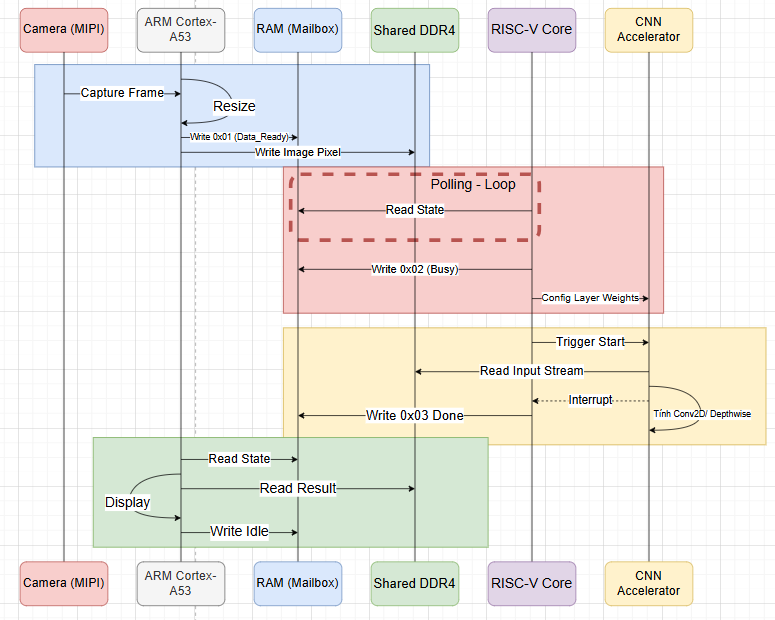
\includegraphics[width=1\textwidth]{images/design/flow.png}
    \caption{Sơ đồ quy trình}
    \label{fig:sequence_diagram}
\end{figure}